Table~\ref{table:topicManMan} displays aspects and sentiments after analyzing user reviews using our approach. Due to space limit, the table only shows results from \enquote{Man Man} application. In the table, the number of positive and negative sentences are also shown to give developers a sense of how often aspects were mentioned in user reviews. Figure~\ref{fig:graphmanman} visualizes the results from Table~\ref{table:topicManMan} with a graph and sorts aspects by sentiment scores. 

The sentiment scores shown in Table~\ref{table:topicManMan} has the highest positive and negative scores of 0.5153 and -0.5156, respectively. Upon examining SentiWordNet, we find that highest \textit{Pos} and \textit{Neg} scores are both 0.75 since the \textit{Obj} score is always non-zero. Since we use averages and absolute maximums when assigning scores to words and sentences, resulting sentiment scores for aspects should be in the range of [-0.75,0.75]. Thus, we can categorize the resulting scores to \textit{low}, \textit{medium}, \textit{high} when absolute scores are [0,0.25), [0.25, 0.5), [0.5,0.75], respectively. Hence, the sentiment score of 0.5153 and -0.5156 in Table~\ref{table:topicManMan} can be considered high positive and high negative. 

\begin{table}[h]
	\caption{20 topics/aspects discovered from Man Man user reviews}
	\label{table:topicManMan}
	\centering
	\begin{tabular}{|l|r|
			r|r|
		}
		\hline
		\multicolumn{1}{|c|}{\multirow{2}{*}{\textbf{Topic/Aspect}}}
		& \multicolumn{1}{|c|}{\multirow{2}{*}{\textbf{Sentiment}}}
		& \multicolumn{2}{|c|}{\textbf{Sentences}}
%		& \multicolumn{1}{|c|}{\textbf{\# Neg. Sentences}}
		\\
		\cline{3-4}
		\multicolumn{1}{|c|}{}
		& \multicolumn{1}{|c|}{}
		& \multicolumn{1}{|c|}{\textbf{\# Pos.}}
		& \multicolumn{1}{|c|}{\textbf{\# Neg.}}
		\\
		\hline
		{- {\selectlanguage{thai}เปลี่ยน ภาษา} <change language>} & 0.2770 
		& 35 & 9 
		\\
		\hline
		{+ {\selectlanguage{thai}พัฒนา ยอด} <develop great>} & 0.2666 
		& 47 & 6 
		\\
		\hline
		{- sticker {\selectlanguage{thai}หน่อย ขยาย} <sticker slightly expand>} & 0.2046 
		& 36 & 15 
		\\
		\hline
		{+ {\selectlanguage{thai}สะดวก สวย} <bueaty comfort>} & 0.3926 
		& 84 & 13 
		\\
		\hline
		{+ {\selectlanguage{thai}สายตา ขนาด ใหญ่} <sight size big>} & 0.5153 
		& 143 & 26 
		\\
		\hline
		{- {\selectlanguage{thai}ยกเว้น ทำนาย} <except predict>} & 0.2315 
		& 19 & 2 
		\\
		\hline
		{- {\selectlanguage{thai}ปรับปรุง ยาก} <update hard>} & 0.2035
		 & 17 & 11 
		 \\
		\hline
		{- {\selectlanguage{thai}ปุ่ม หาย} <button missing>} & -0.5156 
		& 49 & 23 
		\\
		\hline
		{+ {\selectlanguage{thai}ชอบ แม่น} <like accurate>} & 0.3926 
		& 142 & 14 
		\\
		\hline
		{+ {\selectlanguage{thai}สุดยอด ลอง} <topmost try>} & 0.3926 
		& 145 & 12 
		\\
		\hline
		{- {\selectlanguage{thai}แป้น รวน} <keyborad error>} & -0.3352 
		& 24 & 9 
		\\
		\hline
		{- {\selectlanguage{thai}แก้ไข สี} <correct color>} & 0.2167 
		& 40 & 15 
		\\
		\hline
		{+ {\selectlanguage{thai}พิมพ์ ง่าย} <type easy>} & 0.5153 
		& 201 & 12 
		\\
		\hline
		{- {\selectlanguage{thai}เสียง เสียดาย} <sound deplore>} & 0.4066
		 & 17 & 4 
		 \\
		\hline
		{- {\selectlanguage{thai}ปรับ ขนาด ค้าง} <adjust size stuck>} & 0.5153 
		& 63 & 13 
		\\
		\hline
		{+ {\selectlanguage{thai}ปุ่ม แจ่ม ซับซ้อน} <button bright complicate>} & -0.5156 
		& 30 & 17 
		\\
		\hline
		{- {\selectlanguage{thai}เพิ่ม อิโมจิ} <add emoji>} & 0.4066 
		& 35 & 1 
		\\
		\hline
		{- {\selectlanguage{thai}เดา คำ} <guess word>} & -0.5156 
		& 44 & 9 
		\\
		\hline
		{+ {\selectlanguage{thai}พิมพ์ พลาด} <type miss>} & 0.5153 
		& 68 & 11 
		\\
		\hline
		{+ {\selectlanguage{thai}แป้น ใหญ่} <keyboard big>} & 0.3396 
		& 82 & 13 
		\\
		\hline
	\end{tabular}
\end{table}

\begin{figure}
	\centering
	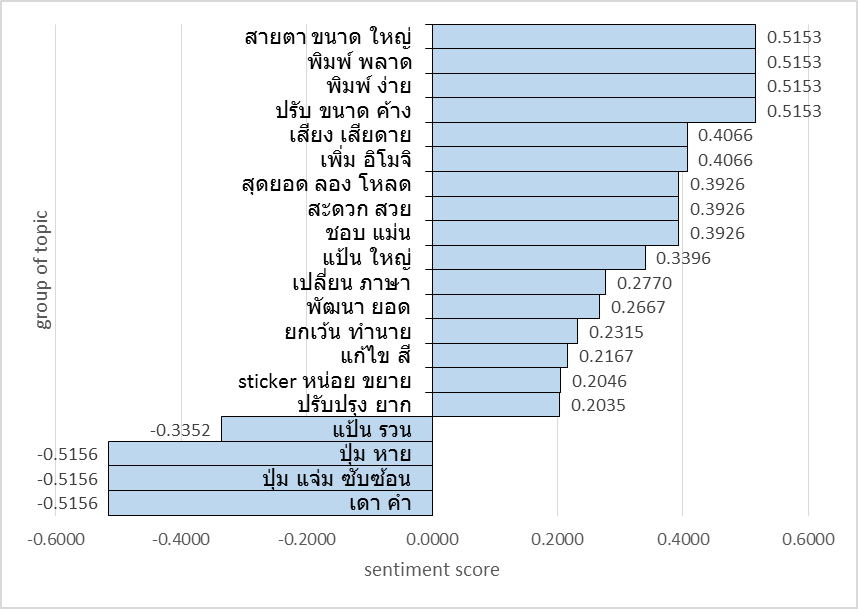
\includegraphics[width=0.9\linewidth]{graphmanman}
	\caption{Sentiment scores for topics/aspects from Man Man user reviews}
	\label{fig:graphmanman}
\end{figure}

%\begin{table}[h]
%	\caption{Evaluation results for sentence-level sentiments}
%	\label{table:f-measureSenti}
%	\centering
%	\begin{tabular}{|l|r|r|r|r|}
%		\hline
%		\multicolumn{1}{|c|}{\textbf{Application}} &
%		\multicolumn{1}{|c|}{\textbf{Precision}} &
%		\multicolumn{1}{|c|}{\textbf{Recall}} &
%		\multicolumn{1}{|c|}{\textbf{F-Measure}} &
%		\multicolumn{1}{|c|}{\textbf{Accuracy}} \\
%		\hline
%		Man Man & 0.5028 & 0.3189 & 0.3570 & 0.6110\\
%		\hline
%		H-TV & 0.5208 & 0.2889 & 0.3366 & 0.4837 \\
%		\hline
%		K-Mobile & 0.4535 & 0.2810 & 0.3240 & 0.5153 \\
%		\hline
%	\end{tabular}
%\end{table}

\begin{table}[!htbp]
	\caption{Evaluation results for sentiment analysis of extracted aspects}
	\label{table:f-measureTopic}
	\centering
	\begin{tabular}{|l|r|r|r|r|}
		\hline
		\multicolumn{1}{|c|}{\textbf{Application}} & 
		%\multicolumn{1}{|c|}{\multirow{2}{*}{application}} & 
		%\multicolumn{4}{|c|}{Topic} \\
		%\cline{2-5}
		%\multicolumn{1}{|c|}{} &
		\multicolumn{1}{|c|}{\textbf{Precision}} &
		\multicolumn{1}{|c|}{\textbf{Recall}} &
		\multicolumn{1}{|c|}{\textbf{F-Measure}} &
		\multicolumn{1}{|c|}{\textbf{Accuracy}} \\
		\hline
		Man Man & 
		%0.7188 
		0.6250
		& 
		0.5808
		%0.6538 
		& 
		0.6021
		%0.6848 
		& 
		0.55
		%0.55
		\\
		\hline
		H-TV & 0.5252 & 0.5333 & 0.5293 & 0.5\\
		\hline
%		K-Mobile & 0.2368 & 0.45 & 0.3103 & 0.45\\
%		\hline
	\end{tabular}
\end{table}

%We evaluated our approach by asking one person not related our research to manually label sentiments whether a sentence is positive, negative, or neutral. This information is used as truth values to calculate precision, recall, and accuracy. Table~\ref{table:f-measureSenti} shows evaluation results of sentiment analysis on a sentence level.

We evaluated our approach by calculating precision, recall, F-measure, and accuracy using truth values from data labeled manually by one person not related to our research. To manually label data, the person was given aspects/topics generated from LDA in the topic modeling step and then labeled each aspect/topic with either positive or negative sentiment. Sentiment scores are not evaluated since it is highly subjective and can be difficult to analyze accuracy. Table~\ref{table:f-measureTopic} shows the evaluation results. The average F-measure from both applications is 0.6071. 

We have not evaluated whether the LDA produced accurate topics/aspects. For topic modeling, accuracy evaluation is very subjective and time-consuming. Different persons may have very different points of view on how to identify topics/aspects in large amount of data.  Since the LDA technique is widely known and used for topic modeling, we assume for now that results from LDA is acceptably accurate. Future work can be done to evaluate this step using similar human-intensive process as in Gunzmam and Laalej's work~\cite{userslikefeature}.

\subsection*{Limitation and Possible Future Works}
Our work still has some limitations such as limitations in word segmentations of informal texts, slangs, and misspelled words. This causes LEXiTRON and SentiWordNet not being able to find translations nor sentiment scores. Moreover, some words have several meanings, and LEXiTRON returns several translations. Thus, we do not get precise meanings nor precise sentiment scores. Possible future work is to create a Thai sentiment lexical resource to help Thai researchers perform sentiment analysis easier and more accurate.

For topic modeling, our work fixes a number of topics and therefore are not flexible or dynamic enough. For future work, we can allow the number to be configurable or determined dynamically from additional information extracted from applications such as a list of features or application size.

The evaluation process is still not ideal since only one person creates truth values. We will ask more persons to label data as our future work. More mobile applications can also be analyzed to expand our case studies. We can also make the approach into a tool where users specify a name of a mobile application and let the tool analyze and display results.


% An example of a double column floating figure using two subfigures.
% (The subfig.sty package must be loaded for this to work.)
% The subfigure \label commands are set within each subfloat command,
% and the \label for the overall figure must come after \caption.
% \hfil is used as a separator to get equal spacing.
% Watch out that the combined width of all the subfigures on a 
% line do not exceed the text width or a line break will occur.
%
%\begin{figure*}[!t]
%\centering
%\subfloat[Case I]{\includegraphics[width=2.5in]{box}%
%\label{fig_first_case}}
%\hfil
%\subfloat[Case II]{\includegraphics[width=2.5in]{box}%
%\label{fig_second_case}}
%\caption{Simulation results for the network.}
%\label{fig_sim}
%\end{figure*}
%
% Note that often IEEE papers with subfigures do not employ subfigure
% captions (using the optional argument to \subfloat[]), but instead will
% reference/describe all of them (a), (b), etc., within the main caption.
% Be aware that for subfig.sty to generate the (a), (b), etc., subfigure
% labels, the optional argument to \subfloat must be present. If a
% subcaption is not desired, just leave its contents blank,
% e.g., \subfloat[].


% An example of a floating table. Note that, for IEEE style tables, the
% \caption command should come BEFORE the table and, given that table
% captions serve much like titles, are usually capitalized except for words
% such as a, an, and, as, at, but, by, for, in, nor, of, on, or, the, to
% and up, which are usually not capitalized unless they are the first or
% last word of the caption. Table text will default to \footnotesize as
% the IEEE normally uses this smaller font for tables.
% The \label must come after \caption as always.
%
%\begin{table}[!t]
%% increase table row spacing, adjust to taste
%\renewcommand{\arraystretch}{1.3}
% if using array.sty, it might be a good idea to tweak the value of
% \extrarowheight as needed to properly center the text within the cells
%\caption{An Example of a Table}
%\label{table_example}
%\centering
%% Some packages, such as MDW tools, offer better commands for making tables
%% than the plain LaTeX2e tabular which is used here.
%\begin{tabular}{|c||c|}
%\hline
%One & Two\\
%\hline
%Three & Four\\
%\hline
%\end{tabular}
%\end{table}


%\begin{table*}[h]
%	\caption{example of result after pass POS tagger process}
%	\label{table:POSEx}
%	\centering
%	\begin{tabular}{|l|l|l|}
%		\hline
%		\multicolumn{1}{|c|}{sentense} &
%		\multicolumn{1}{|c|}{word segmentation} &
%		\multicolumn{1}{|c|}{POS}\\
%		\hline
%		ใช้ได้ดีครับ & 
%		ใช้ได้|ดี|ครับ| & 
%		ใช้ได้/npn ดี/vi ครับ/aff \\
%		\hline
%		เยี่ยม ดี เลิศ & 
%		เยี่ยม|ดี|เลิศ| & 
%		เยี่ยม/vt ดี/adv เลิศ/adv \\
%		\hline
%		พักหลังนี่อัพบ่อยนะครับ & 
%		พัก|หลัง|นี่|อัพบ่อย|นะ|ครับ| & 
%		พัก/vi หลัง/adj นี่/pdem อัพบ่อย/npn นะ/part ครับ/aff \\
%		\hline
%		ชอบค่ะใช้ง่าย มีตัวการ์ตูนให้ด้วย & 
%		ชอบ|ค่ะ|ใช้|ง่าย|มี|ตัว|การ์ตูน|ให้|ด้วย| & 
%		ชอบ/vt ค่ะ/aff ใช้/vt ง่าย/adv มี/vt ตัว/ncn การ์ตูน/ncn ให้/vpost ด้วย/adv \\
%		\hline
%		เรียบง่ายแต่ใช้ได้ดีจริงๆครับชอบมาก & 
%		เรียบง่าย|แต่|ใช้ได้|ดี|จริงๆ|ครับ|ชอบมาก| & 
%		เรียบง่าย/vi แต่/conj ใช้ได้/npn ดี/vi จริงๆ/adv ครับ/aff ชอบ/vt มาก/adv \\
%		\hline
%		ดีมากครับ สะดวกดีแม่นสุดยอด & 
%		ดีมาก|ครับ|สะดวก|ดี|แม่น|สุดยอด| & 
%		ดีมาก/npn ครับ/aff สะดวก/vi ดี/adv แม่น/vt สุดยอด/adj \\
%		\hline
%	\end{tabular}
%\end{table*}

